%
% betaplot.tex -- slide template
%
% (c) 2021 Prof Dr Andreas Müller, OST Ostschweizer Fachhochschule
%
\bgroup
\begin{frame}[t]
\setlength{\abovedisplayskip}{5pt}
\setlength{\belowdisplayskip}{5pt}
\frametitle{Beta-Verteilungen}
\begin{center}
\begin{tikzpicture}[>=latex]

\only<1>{
\begin{scope}
	\clip (-7,-3.2) rectangle (7,3.2);
	\node at (0,-6.5) {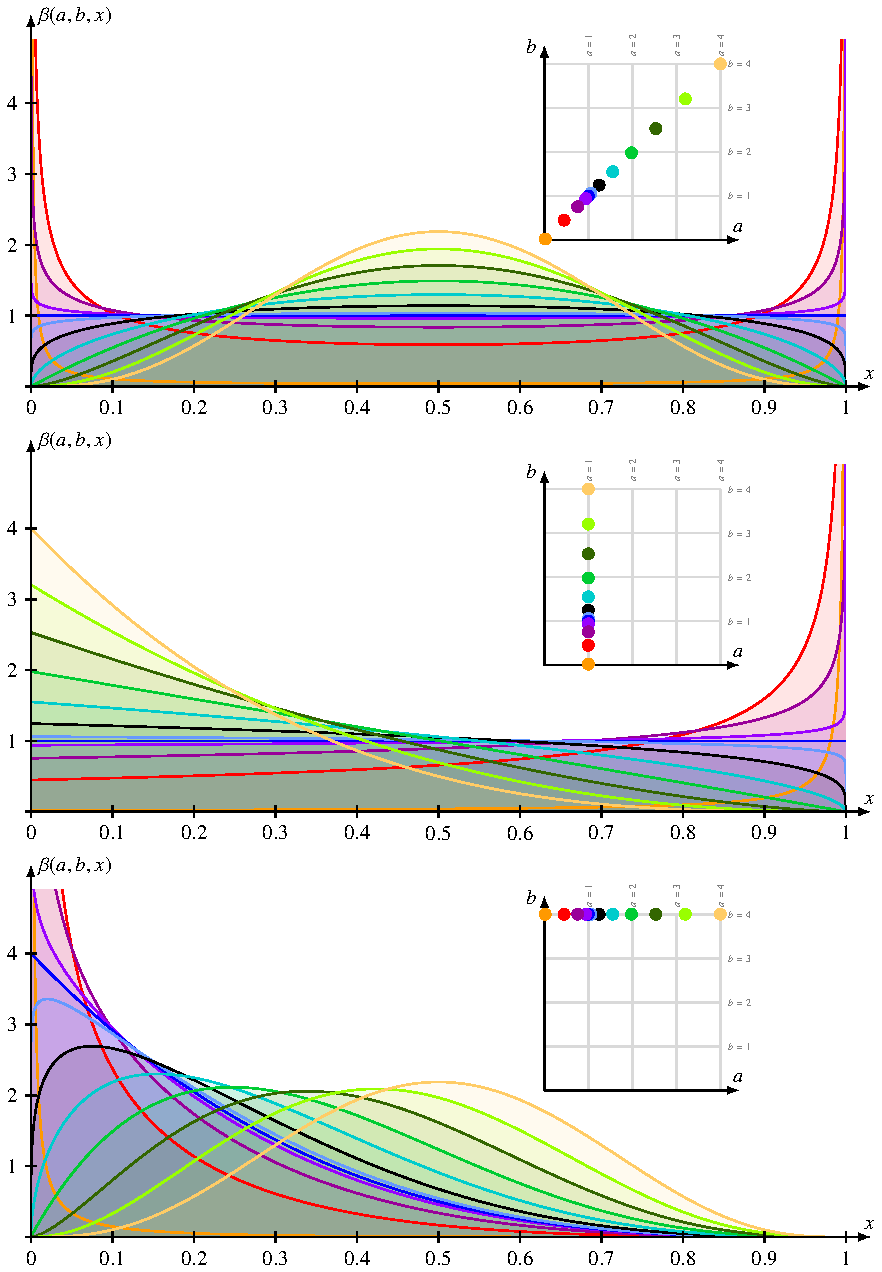
\includegraphics[width=13.5cm]{../../buch/chapters/040-rekursion/images/beta.pdf}};
\end{scope}
}

\only<2>{
\begin{scope}
	\clip (-7,-3.2) rectangle (7,3.2);
	\node at (0,-0) {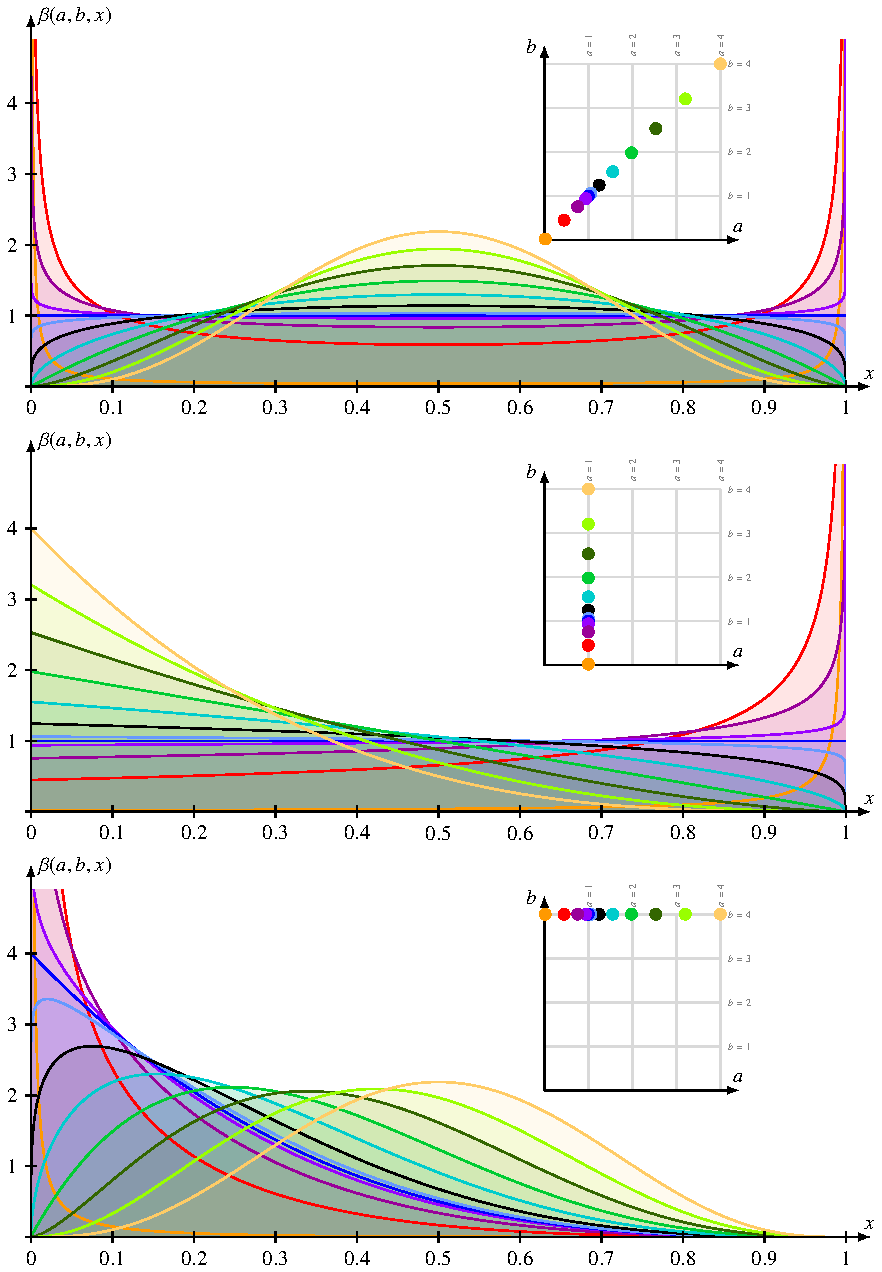
\includegraphics[width=13.5cm]{../../buch/chapters/040-rekursion/images/beta.pdf}};
\end{scope}
}

\only<3>{
\begin{scope}
	\clip (-7,-3.2) rectangle (7,3.2);
	\node at (0,6.5) {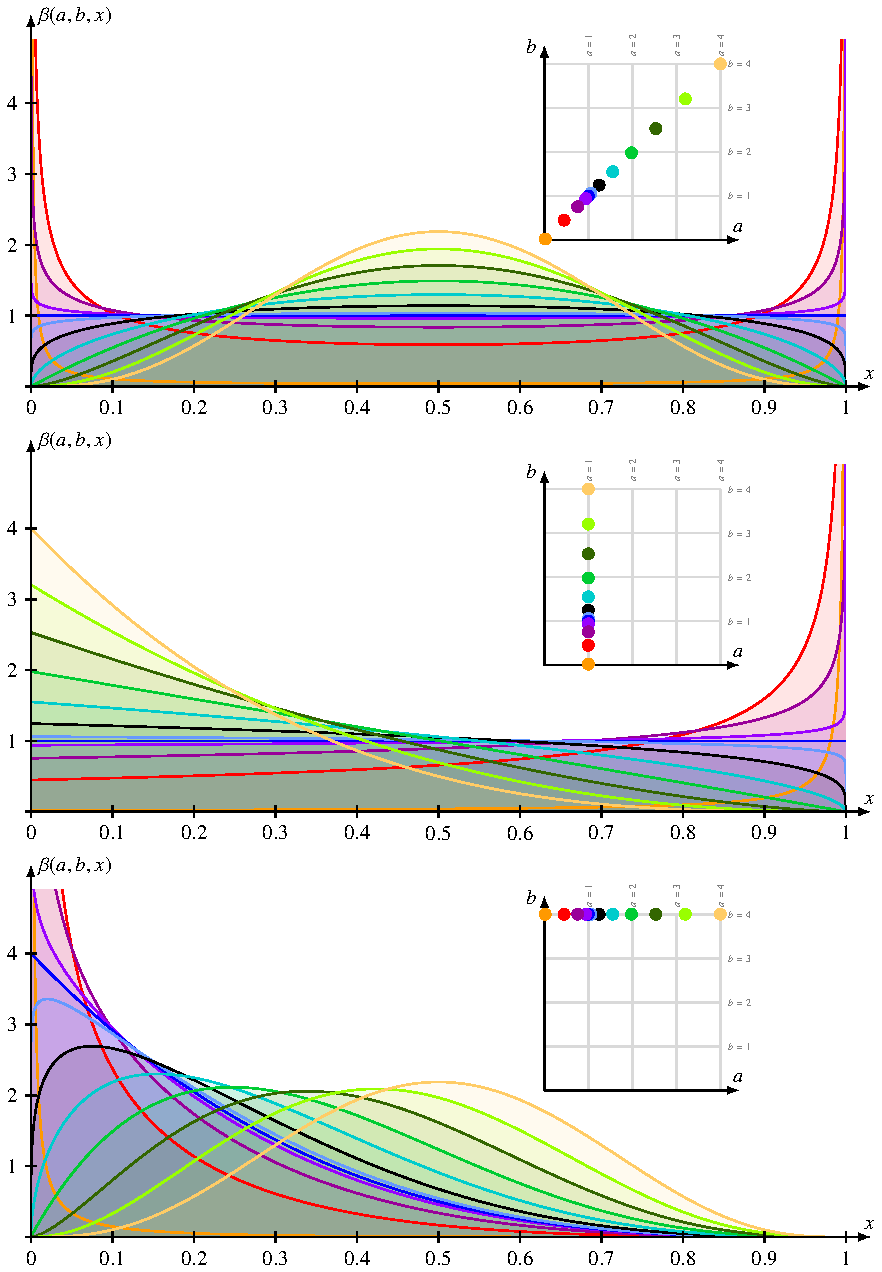
\includegraphics[width=13.5cm]{../../buch/chapters/040-rekursion/images/beta.pdf}};
\end{scope}
}

\end{tikzpicture}
\end{center}
\end{frame}
\egroup
